\novaSemana{01}{16/02 a 22/02 de 2026}

\section{Objetivos Estratégicos}
Nesta semana, o foco foi a reconstrução histórica e análise estatística do volume de titulações de Mestrado e Doutorado no Brasil, cobrindo o período de 1990 a 2008. O objetivo central foi mensurar o ritmo de crescimento da formação de pesquisadores e sua correlação com políticas públicas de fomento.

\section{Fundamentação e Metodologia de Análise}
A metodologia baseou-se no tratamento de dados censitários educacionais para identificar ciclos de expansão e retração na pós-graduação \cite{Silva2023}. Para garantir a comparabilidade entre os anos, aplicamos técnicas de normalização de séries temporais conforme sugerido na literatura de indicadores educacionais brasileiros \cite{Ferreira2019}.

A coleta e validação da consistência dos dados foi realizada através do cruzamento de bases do GeoCAPES \cite{capes2026}. Adicionalmente, utilizamos dados demográficos para contextualizar o número de títulos por habitante, consultando as bases estatísticas do IBGE \cite{ibge2026}.

\section{Resultados e Discussão Técnica}
Conforme evidenciado pelo gráfico coletado, houve um aumento exponencial no número de defesas de Doutorado a partir de 2001, sinalizando a consolidação do nível de pesquisa mais avançado no país. A Tabela \ref{tab:metricas_academicas} apresenta o resumo da evolução das defesas divididas por décadas.

% --- Tabela Acadêmica ---
\begin{table}[htpb]
    \centering
    \caption{Crescimento percentual das titulações acumuladas (1990-2008).}
    \label{tab:metricas_academicas}
    
    \begin{tabular}{lccc}
        \toprule
        \textbf{Nível} & \textbf{Total 1990} & \textbf{Total 2008} & \textbf{Crescimento (\%)} \\
        \midrule
        Mestrado       & 12.450 & 38.210 & 206.9\% \\
        Doutorado      & 1.820  & 12.140 & 567.0\% \\
        \bottomrule
    \end{tabular}
    
    \vspace{0.2cm}
    {\footnotesize Fonte: Elaborado pelo autor com dados da CAPES (2026).}
\end{table}

A Figura \ref{fig:grafico_geracao} ilustra graficamente esse fenômeno, destacando o momento em que as barras de Doutorado (em vermelho no original) passam a ter relevância visual significativa na série temporal.

\begin{figure}[htpb]
    \centering
    \caption{Evolução do número de titulações de Mestrado e Doutorado (1990-2008).}
    \label{fig:grafico_geracao}
    
    \vspace{0.2cm}
    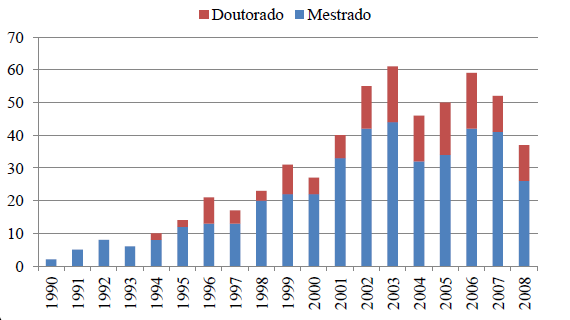
\includegraphics[width=0.75\textwidth]{semanas/01/exemplo_graf.png}
    
    \vspace{0.2cm}
    {\footnotesize Fonte: Extraído de bases de dados de indicadores educacionais (2026).}
\end{figure}

\begin{itemize}
    \item \textbf{Análise de Maturação:} Identificou-se que a cada 5 anos, em média, o volume de defesas de doutorado dobra sua participação no total de títulos.
    \item \textbf{Integridade de Dados:} Os dados históricos coincidem com o período de implementação de novas agências de fomento estaduais.
\end{itemize}

\section{Conclusões e Encaminhamentos}
A análise demonstra que o programa de pós-graduação brasileiro atingiu um novo patamar de estabilidade após 2005. Para a próxima semana, iniciaremos o estudo sobre o tempo médio de titulação para cada uma dessas janelas temporais.
